% !TEX root = main.tex
% Main text: abstract through conclusion. Proofs are in the appendix; numerical checks in Paper2/checks/.
\begin{abstract}
Two training distributions can share every marginal and the Bayes predictor, differ in pairwise correlations by $O(1/N)$ and lie within a vanishing
total-variation distance, yet make gradient training of the same attention model polynomially slower. We prove this for a one-block attention--ReLU Transformer whose
reduced dynamics are derived from its matrices. The mechanism is credit cancellation: attention reads every prefix position, so correlations of order
$1/N$ between the source and the other positions, invisible one at a time, add up and cancel the gradient credit reaching the rule.
With independent context the routing time is $\Theta(N\log(1+\varepsilon^{-2}))$ from initialization scale $\varepsilon$; with cancelled credit it is $\Theta(N/\varepsilon)$,
and over-cancellation stops learning entirely below an exact initialization barrier. The cancellation can be made distributional, so that no function
of what uniform attention reads carries rule credit; a single earlier step that displays the negation of the current state suffices.
Corrupted chain-of-thought supervision is our motivating case: a causal error process with a constant fraction of wrong steps produces the delay at every supervised position,
while independent errors only rescale time by $1/(1-2\eta)$.
A clean fraction $\lambda$ of the order of $\varepsilon$ already removes the bottleneck. When every matrix entry trains under cross-entropy,
the cancelled law still keeps the network within distance $\varepsilon$ of its structured initialization for time $\Omega(1/\varepsilon)$.
Exact population experiments check every rate; from fully random initialization the laws separate in reliability rather than speed.
\end{abstract}

\begin{keywords}%
attention, gradient flow, training dynamics, credit assignment, saddle escape, chain-of-thought supervision%
\end{keywords}

% ===================================================================
\section{Introduction}
\label{sec:intro}

When can two data distributions that are nearly indistinguishable train a network at very different speeds?
We give an exact answer for attention. An attention head that must learn where to look reads all $N$ prefix positions at once.
If each of them correlates with the target-relevant position by only $-1/(N-1)$, no marginal or Bayes predictor changes, but their sum cancels the
gradient credit that would teach the network its rule. The network then sits near its initialization for a time of order $1/\varepsilon$
instead of $\log(1/\varepsilon)$.

\paragraph{A saddle made by the data.}
Slow escape from small initialization is familiar from deep linear networks, where a product of small factors creates a saddle
\citep{saxe2014exact,shamir2019exponential}. The saddle here has a different origin. Our model has the same depth under both laws and the same
source--target correlation; what differs is how the other positions correlate with the source. The cancellation turns the linear growth of a
conserved primitive into quadratic growth, and that changes the escape time from logarithmic to inverse in $\varepsilon$.
Weak-gradient analyses \citep{shalevshwartz2017failures,abbe2025parities} relate slow learning to weak target correlation; here the target correlation is fixed
and only the sum over attended positions cancels.

\paragraph{Corrupted chain-of-thought as the motivating case.}
Reasoning traces used for supervision can contain incorrect intermediate steps \citep{havrilla2024noise,zhou2024noisyrationales},
and a model can still learn the correct rule when it remains the most likely next step \citep{natarajan2013noisy,patrini2017loss}.
For modulo-two counting the clean step is $x_{i+1}=b_{i+1}x_i$; a corrupted trace shows $x_{i+1}=b_{i+1}x_i\xi_{i+1}$ with $\Pr(\xi_{i+1}=-1)=\eta$.
At uniform attention the rule gradient factorizes into reliability and contextual credit:
\[
 -\pd{\mathcal L}{r_1}
 =\frac{r_2}{2N}
 \underbrace{(1-2\eta)}_{\text{label reliability }\gamma}
 \underbrace{\left(1+\sum_{j=1}^{N-1}\E[x_Nx_j]\right)}_{\text{contextual credit }\kappa}.
\]
Independent errors lower $\gamma$, which only rescales time. Errors that make earlier steps anti-correlate with the current state lower $\kappa$,
which changes the order of the routing time. A single earlier step that displays the negation of the current state is enough.
Such steps arise when slips are more frequent where the correct state agrees with most earlier steps, so that wrong steps keep the displayed
history balanced; \cref{thm:causal} shows that this error process produces exact cancellation at every supervised step.

\begin{figure}[t]
\centering
\resizebox{\linewidth}{!}{% Conceptual figure: what uniform attention reads under the two matched laws.
\begin{tikzpicture}[>=Stealth, font=\small,
  src/.style={rectangle, rounded corners=2pt, draw=royalazure!80!black, fill=royalazure!14, minimum width=9mm, minimum height=6mm, inner sep=1pt},
  dec/.style={rectangle, rounded corners=2pt, draw=black!45, fill=black!5, minimum width=9mm, minimum height=6mm, inner sep=1pt},
  anti/.style={rectangle, rounded corners=2pt, draw=red!70!black, fill=red!10, minimum width=9mm, minimum height=6mm, inner sep=1pt},
  qry/.style={rectangle, rounded corners=2pt, draw=orange!80!black, fill=orange!14, minimum width=9mm, minimum height=6mm, inner sep=1pt}]

% (a) independent decoys
\begin{scope}
  \node[font=\small\bfseries, anchor=west] at (-0.2,2.25) {(a) independent law $\mathcal D_1$};
  \node[dec] (d1a) at (0,1.2) {$x_1$};
  \node[dec] (d2a) at (1.15,1.2) {$x_2$};
  \node at (2.15,1.2) {$\cdots$};
  \node[dec] (d3a) at (3.15,1.2) {$x_{N-1}$};
  \node[src] (sa) at (4.45,1.2) {$x_N$};
  \node[qry] (qa) at (2.2,-0.55) {$b\ \to\ y$};
  \foreach \d in {d1a,d2a,d3a} { \draw[->, black!45] (\d.south) -- (qa.north); }
  \draw[->, thick, royalazure] (sa.south) -- (qa.north);
  \node[font=\scriptsize, align=center, text=black!70] at (2.2,-1.45)
     {decoys independent of $x_N$:\quad $\E[y b\,x_j]=0$};
  \node[font=\scriptsize, align=center, text=royalazure] at (2.2,-2.05)
     {rule credit at uniform attention $=\frac{\gamma}{N}\cdot 1$};
\end{scope}

% (b) one anti-copy at a random position
\begin{scope}[shift={(7.2,0)}]
  \node[font=\small\bfseries, anchor=west] at (-0.2,2.25) {(b) anti-copy law $\mathcal D_0$};
  \node[dec] (d1b) at (0,1.2) {$x_1$};
  \node[anti] (d2b) at (1.15,1.2) {$-x_N$};
  \node at (2.15,1.2) {$\cdots$};
  \node[dec] (d3b) at (3.15,1.2) {$x_{N-1}$};
  \node[src] (sb) at (4.45,1.2) {$x_N$};
  \node[qry] (qb) at (2.2,-0.55) {$b\ \to\ y$};
  \foreach \d in {d1b,d3b} { \draw[->, black!45] (\d.south) -- (qb.north); }
  \draw[->, red!70!black] (d2b.south) -- (qb.north);
  \draw[->, thick, royalazure] (sb.south) -- (qb.north);
  \node[font=\scriptsize, text=red!70!black] at (1.15,1.75) {random position};
  \node[font=\scriptsize, align=center, text=black!70] at (2.2,-1.45)
     {each decoy: $\E[y b\,x_j]=-\frac{\gamma}{N-1}$;\quad multiset $\{x_j\}$ independent of $x_N$};
  \node[font=\scriptsize, align=center, text=red!70!black] at (2.2,-2.05)
     {rule credit at uniform attention $=\frac{\gamma}{N}\bigl(1-(N-1)\cdot\frac{1}{N-1}\bigr)=0$};
\end{scope}
\end{tikzpicture}
}
\caption{Two laws with the same marginals and Bayes predictor, read by uniform attention. The query holds the current letter $b$ and
must predict the displayed successor $y=b x_N \xi$, where $\xi$ is an error independent of everything else. In (a) the prefix
positions are independent of the source. In (b) one prefix position, chosen uniformly at random, displays $-x_N$, so each position
correlates with the source by $-1/(N-1)$. This leaves every marginal and the Bayes predictor unchanged, but the $N-1$ positions are read
together and cancel the source's contribution (\cref{lem:credit}); the multiset of displayed values is even independent of $x_N$ (\cref{lem:matched}).}
\label{fig:cancel}
\end{figure}

\paragraph{Two kinds of result.} The obstruction is proved in two complementary forms. The first is general: under the cancelled law the label is
independent of everything uniform attention reads (\cref{lem:matched}), so near the structured initialization no parameter of a full-matrix network
receives rule signal, and cross-entropy flow on every matrix entry needs time $\Omega(1/\varepsilon)$ to leave an $\varepsilon$-ball (\cref{thm:fullmatrix}).
The second is exact: in the four-scalar model a conserved quantity solves the coupled flow, giving routing times of the same order in $\varepsilon$, the barrier
for over-cancellation and the dependence on the clean fraction (\cref{thm:separation,cor:dilution}). \Cref{thm:causal} then produces the cancelled law
from an error process that acts one step at a time.

\paragraph{Contributions.}
\begin{enumerate}[leftmargin=*,itemsep=2pt,topsep=2pt]
\item \textbf{Matched laws, separated training times} (\cref{lem:matched,thm:separation}). Laws with the same error rate, marginals and Bayes predictor,
at total-variation distance $O(N^{-1/2})$, give routing times $\Theta((N/\gamma)\log(1+\varepsilon^{-2}))$ and $\Theta(N/(\gamma\varepsilon))$ under correlation loss,
with absolute constants, from an exact conserved quantity. Over-cancellation has an exact barrier, and cross-entropy keeps both orders for escape.
\item \textbf{Distributional cancellation} (\cref{lem:matched,cor:uniform}). Under the anti-copy law the label is independent of everything uniform attention reads,
so every non-attention parameter of any one-block network sees pure label noise at the start; only routing can break the plateau.
\item \textbf{A dose--response law for clean data} (\cref{cor:dilution}). A fraction $\lambda$ of traces without cancellation gives
$\Theta((N/\gamma)\min\{1/\varepsilon,(1+\log(1+\lambda/\varepsilon))/\lambda\})$: the bottleneck disappears once $\lambda$ exceeds the initialization scale.
\item \textbf{The plateau survives full-matrix training} (\cref{thm:fullmatrix}). With every query, key, value, output, MLP and readout entry trained by
cross-entropy, the cancelled law gives $|\E[yz]|=O(\varepsilon^3)$ on an $\varepsilon$-ball around the structured initialization, which takes time $\Omega(1/\varepsilon)$ to leave.
\item \textbf{Wrong CoT steps can cause it} (\cref{thm:causal}). A causal error kernel with local error rate $\eta$ and a constant fraction of wrong transitions
produces cancellation at every supervised step, with the correct step still Bayes optimal.
\end{enumerate}

\paragraph{The scope of the claim.} The theorems concern a one-block attention--ReLU network with specified matrix directions and four trained scalars,
derived exactly from its matrices (\cref{prop:realization}); \cref{thm:fullmatrix} lifts the lower bound to full-matrix training near the same initialization.
The separation is in the initialization scale at fixed $N$, and complete cross-entropy routing is verified numerically rather than proved.
From fully random initialization, and in a standard Transformer, the delay does not appear in the same form (\cref{sec:numerics}).

% ===================================================================
\section{Model and corruption laws}
\label{sec:setup}
\paragraph{Notation and prediction task.}
A prediction reads displayed signs $\bm x_{<N+1}=(x_1,\ldots,x_N)$ and an instruction $b\in\{-1,1\}$, and predicts $y\in\{-1,1\}$.
The last visible state $x_N$ is the source and positions $j<N$ are decoys; in modulo-two counting the clean transition is $y=b x_N$.
We write $\eta$ for the error probability, $\gamma=1-2\eta$, $\varepsilon$ for the initialization scale and $\kappa$ for the cancellation coefficient;
$\alpha(q)$ is source attention, $\phi(q)$ the effective credit and $F(q)$ the primitive of the invariant, with primes for derivatives in $q$.

\begin{definition}[Matched prediction laws]
\label{def:law}
A law of $(\bm x_{<N+1},b,y)$ has error probability $\eta$ if
$\Pr(y\ne b x_N\mid x_N,b)=\eta$; its margin is $\gamma=1-2\eta$.
Two laws are matched when they have the same $\eta$ and the same Bayes predictor given $(\bm x_{<N+1},b)$.
\end{definition}

\begin{definition}[The anti-copy law $\Dlaw{\kappa}$]
\label{def:Dkappa}
Fix $N\ge4$, $\eta\in[0,1/2)$, $\kappa\in[-1,1]$, and $\rho=(1-\kappa)/(N-1)$.
Draw the source $x_N$ uniform. Draw the number of anti-copies $M=\lfloor1-\kappa\rfloor+\beta$, where
$\beta\in\{0,1\}$ has $\Pr(\beta=1)=1-\kappa-\lfloor1-\kappa\rfloor$, so that $M\in\{0,1,2\}$ and $\E[M]=1-\kappa$.
Choose $M$ of the $N-1$ decoy positions uniformly at random and set them to $-x_N$; draw the remaining decoys independently and uniformly.
Independently draw $b$ uniform and $\xi\in\{-1,1\}$ with $\Pr(\xi=-1)=\eta$;
set $y=b x_N \xi$ and $\gamma=1-2\eta$.
\end{definition}
Write $\bar w=(1/(N-1))\sum_{j<N}x_j$ for the decoy average.
Every displayed sign is uniform, and $\E[x_N x_j]=-\rho$ for each decoy.
Under $\Dlaw{1}$ the source is independent of the decoys; under $\Dlaw{0}$ exactly one decoy is the anti-copy $-x_N$, at a random position;
under $\Dlaw{-1}$ two are. In chain-of-thought terms, the anti-copy is an earlier step that displays the negation of the current state.
The analysis is not confined to $\kappa=0$: \cref{cor:dilution} covers every $\kappa\in[0,1]$ and keeps the order $1/\varepsilon$ for $\kappa\le c\varepsilon$,
\cref{thm:separation}(iii) covers $\kappa<0$, and \cref{thm:causal} obtains $\kappa=0$ from a causal error process.

\subsection{One-block Transformer and initialization}
\label{sec:architecture}
We use one causal attention head followed by a positionwise, four-unit ReLU MLP, with residual connections and a binary readout.
The theoretical architecture omits layer normalization and dropout. Its query attends to the $N$ preceding state positions;
a fixed type mask excludes the query itself and instruction-only positions. This is a specified one-block Transformer,
with a restricted set of trainable directions. Normalization would change the exact identities below.

The residual stream is seven-dimensional. A state position carries its displayed sign $x_j$, a constant, and a flag for the source ($j=N$)
or a decoy ($j<N$); the query carries the instruction $b$ and the constant. The key reads only the two flags, with trainable weights $q_s$ (source)
and $q_d$ (decoys), so every decoy shares one score; the value reads $x_j$. The MLP has four ReLU units whose first-layer rule weight $r_1$ reads
the attended value and whose fixed gate weight $B$ reads $b$, with bias $-B$; its second layer has rule weight $r_2$ and feeds the readout.
The explicit matrices are in \cref{app:architecture}.

\paragraph{Initialization and training.}
Choose $0<\varepsilon\le1$ and fix the gate scale before training so that
\begin{equation}
 B>\sqrt{\varepsilon^2+\log(N-1)+1+e}.
 \label{eq:gate-bound}
\end{equation}
The trainable parameters and their initialization are
\begin{equation}
 \bm\theta=(q_s,q_d,r_1,r_2)^\top\in\mathbb R^4,\qquad
 \bm\theta(0)=(0,0,\varepsilon,\varepsilon)^\top.
 \label{eq:initialization}
\end{equation}
Thus $\bm w_k(0)=\bm0^\top$, every score is zero, $\alpha_j(0)=1/N$,
and the two MLP factors both start at $\varepsilon$.
All other directions in \cref{eq:attention-matrices,eq:mlp-matrices} are fixed.
We train these four coordinates by population gradient flow in training time $t$, using either loss:
\begin{equation}
 \mathcal L_{\mathrm{corr}}(\bm\theta)=-\frac{1}{2}\E[y z_{\bm\theta}],\qquad
 \mathcal L_{\mathrm{ce}}(\bm\theta)=\E\bigl[\log(1+e^{-y z_{\bm\theta}})\bigr],\qquad
 \frac{d\bm\theta(t)}{dt}=-\nabla_{\bm\theta}\mathcal L(\bm\theta(t)).
 \label{eq:parameter-flow}
\end{equation}
Gradient flow uses the Euclidean metric on the parameter coordinates.
The tied rows contribute through the chain rule; the entries of the matrices are not independent trainable coordinates.
The positional features identify the candidate source, while its attention weight is learned from uniform initialization.

\begin{proposition}[Exact reduction of the one-block network]
\label{prop:realization}
For $b\in\{-1,1\}$ and $|r_1v|<2B$, the network in \cref{eq:attention-block,eq:mlp-matrices} has logit
\begin{equation}
 z=r_1r_2b v.
 \label{eq:model}
\end{equation}
For either population correlation loss or binary cross-entropy, its gradients with respect to the four trainable scalars
are exactly those of \cref{eq:model}. Since all decoys share one score, the attention read is
$v=\alpha(q)x_N+(1-\alpha(q))\bar w$, where
$q=q_s-q_d$ and $\alpha(q)=e^q/(e^q+N-1)$.
\end{proposition}
The proof in \cref{app:network-proof} has three steps: attention, the MLP identity, and the chain rule.

\paragraph{Routing and prediction.}
With $q_1=\log(N-1)$, the routing time is $\Tr:=\inf\{t\ge0:\alpha(q(t))\ge1/2\}$. At $q>q_1$ and $r_1r_2>0$, $x_N v>0$ on every prefix,
so $\operatorname{sign}(z)=b x_N$ is the Bayes prediction. \Cref{eq:gate-bound} keeps the reduction valid through $q=q_1+1$ and through the cross-entropy escape;
correlation loss is unbounded below, so its convergence claims concern prediction.

% ===================================================================
\section{Why credit cancels}
\label{sec:cancel}

\begin{lemma}[Credit cancellation]
\label{lem:credit}
Let a law have clean next-step rule $b x_N$ and reliability $\gamma$, and suppose $\xi:=y b x_N$ is independent of $(\bm x_{<N+1},b)$. For correlation loss at uniform attention, in the model of \cref{eq:model},
\[
 -\pd{\mathcal L}{r_1}=\frac{r_2}{2}\cdot\frac{\gamma\,\kappa}{N},
 \qquad
 \kappa:=1+\sum_{j=1}^{N-1}\E[x_N x_j],
\]
and symmetrically for $r_2$. For $\Dlaw{\kappa}$ the coefficient is the parameter $\kappa$ of \cref{def:Dkappa}; in particular the rule gradient vanishes identically
under $\Dlaw0$, and under $\Dlaw{\kappa}$ with $\kappa<0$ it points away from the rule.
\end{lemma}

The proof separates the source contribution $\gamma/N$ from the decoy contributions
$(\gamma/N)\E[x_N x_j]$. The latter are not fixed by the local prediction law.
For $\Dlaw{\kappa}$ they sum to $-\gamma(1-\kappa)/N$, so $\kappa=0$ cancels the source contribution.
The full proof is in \cref{app:credit-proof}.

\begin{lemma}[Matched laws and distributional cancellation]
\label{lem:matched}
For every $\kappa\in[-1,1]$, $\Dlaw{\kappa}$ and $\Dlaw1$ are matched (\cref{def:law}): both have rule $y=b x_N$, error rate $\eta$,
and Bayes predictor given the prefix $\hat y=b x_N$ with accuracy $1-\eta$. Every displayed value has the uniform marginal under both.
With $S_{N-1}$ a sum of $N-1$ independent uniform signs and $\tau_N=\E|S_{N-1}|/(2(N-1))\le1/(2\sqrt{N-1})$,
\[
 d_{\mathrm{TV}}(\Dlaw{\kappa},\Dlaw1)=(1-\kappa)\,\tau_N\quad(0\le\kappa\le1),\qquad
 d_{\mathrm{TV}}(\Dlaw{\kappa},\Dlaw1)\le\frac{1-\kappa}{2\sqrt{N-2}}\quad(-1\le\kappa\le1).
\]
Under $\Dlaw0$ the multiset $\{x_1,\ldots,x_N\}$ of displayed values is independent of $x_N$, and $y$ is independent of
$(b,\{x_1,\ldots,x_N\})$. Under $\Dlaw1$, $\E[y b x_N]=\gamma$.
\end{lemma}

The matched laws differ by a total-variation distance that vanishes with $N$ and leave every marginal and the Bayes predictor unchanged.
The independence statement does not depend on the architecture after attention.

\begin{corollary}[No rule signal at uniform attention]
\label{cor:uniform}
Let each state position $j$ be embedded as $x_j\bm u+\bm p_j$, where the position features $\bm p_j$ do not depend on the displayed values, and let an attention
layer with uniform weights and a linear value map $V$ produce $\bar{\bm v}=\frac1N\sum_jV(x_j\bm u+\bm p_j)$. Let $g_\psi(b,\bar{\bm v})$ be any measurable map, of any depth,
width, normalization or nonlinearity, with parameters $\psi$. Under $\Dlaw0$, $y$ is independent of $(b,\bar{\bm v})$; hence $\E[y\,g_\psi(b,\bar{\bm v})]=0$ for every $\psi$, and
for any loss the population gradient with respect to $\psi$ equals its gradient when $y$ is replaced by an independent label with the same marginal.
\end{corollary}
\begin{proof}
$\bar{\bm v}=\frac{S}{N}V\bm u+\frac1N\sum_jV\bm p_j$ with $S=\sum_jx_j$, a function of the multiset of displayed values, and \cref{lem:matched} gives that $y$ is independent of
$(b,\{x_1,\ldots,x_N\})$. The expected loss and its gradient in $\psi$ depend only on the joint law of $(y,b,\bar{\bm v})$, which is then a product law.
\end{proof}
So enlarging the MLP or the readout cannot remove the plateau; only the attention scores can move the network off it.
A shared-decoy law cannot do this: if every decoy displays one value $w$, the multiset determines $x_N$.

% ===================================================================
\section{Main optimization result}
\label{sec:dynamics}

Decoys share a score, so the flow depends on the scores only through $q=q_s-q_d$, with
$\alpha(q)=e^q/(e^q+N-1)$. Write
\[
 \phi(q)=(1+\rho)\,\alpha(q)-\rho,\qquad \phi'(q)=(1+\rho)\,\alpha(q)\bigl(1-\alpha(q)\bigr),
\]
so that $\E[y b v]=\gamma\,\phi(q)$ and $\phi(0)=\kappa/N$ by \cref{lem:credit}. The loss is $\mathcal L=-(\gamma/2)r_1r_2\phi(q)$.

\begin{lemma}[Gradient-flow invariant]
\label{lem:invariant}
From \cref{eq:initialization}, correlation-loss gradient flow under $\Dlaw{\kappa}$ keeps $r_1=r_2=:r>0$, $q_s+q_d=0$, and satisfies
\[
 \ddt{r}=\frac{\gamma}{2}\,r\,\phi(q),\qquad \ddt{q}=\gamma\,r^2\phi'(q).
\]
The quantity $r^2-F(q)$ is conserved, where
\[
 F(q)=\int_0^q\frac{\phi(v)}{\phi'(v)}\,dv.
\]
Hence $r(t)^2=\varepsilon^2+F(q(t))$, $q$ is nondecreasing, and whenever $\varepsilon^2+F>0$ on $[0,q_1]$ the routing time is
\begin{equation}
 \Tr=\int_0^{q_1}\frac{dv}{\gamma\,\bigl(\varepsilon^2+F(v)\bigr)\,\phi'(v)}.
 \label{eq:time}
\end{equation}
For $\kappa\in\{0,1\}$, the gap $q_1+1$ is reached in finite time, and prediction is Bayes optimal whenever $q_1<q(t)\le q_1+1$.
\end{lemma}
\emph{Proof idea.} The loss is $-(\gamma/2)r_1r_2\phi(q)$, so $\ddt{r_1}=(\gamma/2)r_2\phi$, $\ddt{r_2}=(\gamma/2)r_1\phi$ and the two score
velocities are opposite; the initial symmetries persist, and the chain rule gives $\tfrac{d}{dt}(r^2-F)=\gamma r^2\phi-(\phi/\phi')\gamma r^2\phi'=0$ (\cref{app:flow-proof}).


The invariant reduces routing to one integral. Under independent contexts $F$ grows linearly near zero;
under cancellation it grows quadratically, keeping the rule near initialization for longer.

\begin{mainresult}
\begin{theorem}[Matched laws, separated routing times]
\label{thm:separation}
Consider the network and Euclidean gradient flow in \cref{sec:architecture}, initialized by \cref{eq:initialization}.
Let $N\ge4$, $\eta\in[0,1/2)$, $\gamma=1-2\eta$, and $0<\varepsilon\le1$.
The laws $\Dlaw{\kappa}$, $\kappa\in[-1,1]$, have the same clean rule, error probability and Bayes predictor,
with $d_{\mathrm{TV}}(\Dlaw{\kappa},\Dlaw1)\le(1-\kappa)/(2\sqrt{N-2})$.
\begin{enumerate}[label=(\roman*),leftmargin=*,itemsep=2pt,topsep=2pt]
\item \emph{Independent context, correlation loss.}
$\displaystyle \Tr(\Dlaw1)=\Theta\!\left(\frac{N}{\gamma}\log(1+\varepsilon^{-2})\right)$.
\item \emph{Exact cancellation, correlation loss.}
$\displaystyle \Tr(\Dlaw0)=\Theta\!\left(\frac{N}{\gamma \varepsilon}\right)$.
The comparison constants in (i)--(ii) are absolute. Both flows reach the Bayes predictor on the gate-valid interval beyond routing.
\item \emph{Over-cancellation, correlation loss.}
For $-1\le \kappa<0$, put $q_0=\log(1-\kappa)$. Then
\[
 \Tr<\infty\quad\Longleftrightarrow\quad \varepsilon^2>-F(q_0).
\]
At or below the barrier, routing fails and $r(t)\to0$.
The limiting gap is the first zero of $\varepsilon^2+F$ below $q_0$, or $q_0$ at equality.
\item \emph{Escape, binary cross-entropy.}
For fixed $N,\gamma$ there is an escape gap $q_{\mathrm{esc}}>0$ such that, for sufficiently small $\varepsilon>0$,
the times to reach $q_{\mathrm{esc}}$ satisfy
\[
 \Tr_{\mathrm{esc}}(\Dlaw1)=\Theta\!\left(\log\!\frac{1}{\varepsilon}\right),\qquad
 \Tr_{\mathrm{esc}}(\Dlaw0)=\Theta\!\left(\frac{1}{\varepsilon}\right),
\]
and the matrix reduction stays valid on the way.
Here the constants and escape gap may depend on $N,\gamma$.
\end{enumerate}
\end{theorem}
\end{mainresult}

For fixed $N$ and $\gamma$, the ratio $\Tr(\Dlaw0)/\Tr(\Dlaw1)$ is of order $1/(\varepsilon\log(1/\varepsilon))$. Both routing times are
linear in $N$: \emph{the separation is in the initialization scale}, not in the prefix length. It becomes a separation in $N$ only if $\varepsilon$ is tied to $N$;
for example $\varepsilon\propto N^{-1/2}$ would give $\Tr(\Dlaw1)\lesssim N\log N$ against $\Tr(\Dlaw0)\gtrsim N^{3/2}$, but we do not claim that this coupling
is what standard initializations produce for the four tied scalars.

\begin{remark}[Reliability only rescales time]
\label{rem:rescaling}
With an independent error sign, $\mathcal L_\eta=(1-2\eta)\mathcal L_0$ under correlation loss, so $T(\eta,\kappa)=T(0,\kappa)/(1-2\eta)$ for every $\kappa$:
independent errors cost a constant factor, while contextual credit changes the order.
\end{remark}

\begin{remark}[Sign-based updates remove the delay]
\label{rem:sign-flow}
The delay comes from the size of the score gradient, $\gamma r^2\phi'(q)$, not from its sign. Under sign flow, $\dot\theta_i=-\operatorname{sign}(\partial_{\theta_i}\mathcal L_{\mathrm{corr}})$
from \cref{eq:initialization}, and for $\kappa\in[0,1]$: $\phi(q)\ge\phi(0)=\kappa/N\ge0$ for $q\ge0$, so $r_1=r_2\ge\varepsilon>0$, both score coordinates move at unit speed,
and $\alpha(q)$ reaches $\frac12$ at time exactly $\frac12\log(N-1)$, for every $\varepsilon$ and $\kappa$. Adam's per-coordinate normalization approximates sign updates,
which is why it removes the separation in \cref{sec:numerics}.
\end{remark}

\begin{corollary}[A small clean fraction removes the bottleneck]
\label{cor:dilution}
For $0\le\lambda\le1$, the mixture of a fraction $\lambda$ of $\Dlaw1$ with $1-\lambda$ of $\Dlaw0$ is $\Dlaw\lambda$.
Under correlation loss, for $0<\varepsilon\le1$,
\[
 \Tr(\Dlaw\lambda)=\Theta\!\left(\frac{N}{\gamma}\min\left\{\frac{1}{\varepsilon},\ \frac{1+\log(1+\lambda/\varepsilon)}{\lambda}\right\}\right)
\]
with absolute constants. A fraction $\lambda\lesssim\varepsilon$ leaves the $1/\varepsilon$ bottleneck in place; $\lambda\gg\varepsilon$ removes it,
and $\lambda=1$ recovers \cref{thm:separation}(i).
\end{corollary}
At $\varepsilon=10^{-3}$ and $N=16$, for example, a clean fraction of $1\%$ cuts the routing time from $44{,}249$ to $10{,}579$, and $10\%$ cuts it to $1{,}924$ (\cref{fig:kappa}).
The proof bounds the primitive by $F(q)\asymp\lambda q+q^2/2$ on $[0,1]$ (\cref{app:dilution}).


\paragraph{Where the delay accumulates.}
Under $\Dlaw0$ the score gap starts at rate $\gamma\varepsilon^2/N$ and $F(q)=q^2/2+O(q^3)$, so the rule stays near its initialization until $q$ is of
order $\varepsilon$, which gives the inverse-initialization delay; under $\Dlaw1$, $F'(0)>0$ and the same integral gives a logarithm. Beyond a fixed score gap the
remaining time is bounded independently of $\varepsilon$. Under over-cancellation $\phi<0$ first shrinks the rule, and the barrier in $F$ decides whether routing escapes (\cref{fig:phase}).

\begin{figure}[t]
\centering
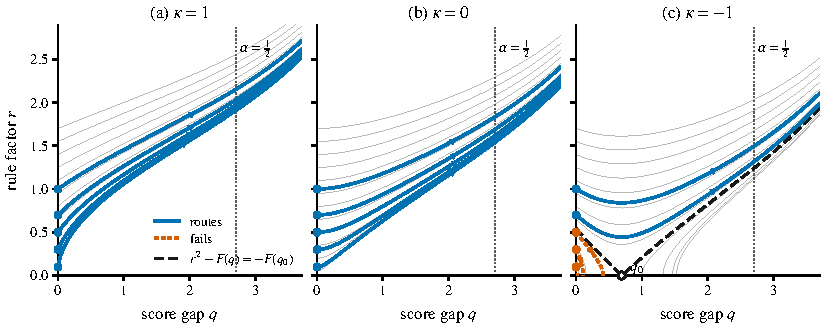
\includegraphics[width=\linewidth]{figures/phase_portrait.pdf}
\caption{Phase portrait of the reduced correlation-loss flow. $N=16$, $\eta=0.1$; grey curves are level sets of the invariant $r^2-F(q)$
(\cref{lem:invariant}), and trajectories start at $(0,\varepsilon)$ for $\varepsilon\in\{0.1,0.3,0.5,0.7,1\}$; the dotted line marks source attention $\alpha=1/2$.
(a)~Under $\Dlaw1$, $F$ is linear near $q=0$ and every trajectory leaves the axis at once; (b)~under $\Dlaw0$, $F(q)=q^2/2+O(q^3)$ and small-$\varepsilon$
trajectories creep along it. (c)~Under over-cancellation the rule first shrinks, and the separatrix $r^2-F(q)=-F(q_0)$ through $(q_0,0)$ divides routing from
collapse, the barrier $\varepsilon^2>-F(q_0)$ of \cref{thm:separation}(iii).}
\label{fig:phase}
\end{figure}


The proofs in \cref{app:routing-proof,app:critical} use one attention estimate, one primitive estimate, and the barrier minimum.

% ===================================================================
\section{Cross-entropy: escaping the bottleneck}
\label{sec:crossentropy}
Theorem~\ref{thm:separation}(iv) concerns the escape from uniform attention at fixed $N,\gamma$.
Cross-entropy preserves the matrix reduction and the score metric, but changes the rule gradient.
\emph{Proof idea.} With $m=r^2$, the exact derivatives give $m(q)=\Theta(\varepsilon^2+q^{2-\kappa})$ and $\ddt q=\Theta(m)$ on a small fixed
interval of $q$, for $\kappa\in\{0,1\}$, so the local hitting time is $\Theta(\int_0^b\frac{dq}{\varepsilon^2+q^{2-\kappa}})$: a logarithm for $\kappa=1$
and $1/\varepsilon$ for $\kappa=0$ (\cref{app:ce-proof}).

\paragraph{Beyond escape.}
For the anti-copy law the attended read takes many values, and at large rule product the cross-entropy score velocity
could in principle change sign before routing. We therefore do not claim complete cross-entropy routing as a theorem.
Numerically it completes in every tested configuration, with the score velocity bounded away from zero along each trajectory,
and the complete-routing times keep the two initialization orders (\cref{tab:network-flow,fig:network-flow}).

% ===================================================================
\section{Full-matrix training: a cross-entropy plateau}
\label{sec:fullmatrix}
\Cref{thm:separation} trains four tied scalars. Could a network whose every matrix entry trains escape the cancellation by learning other features,
other value maps or other attention patterns? Near the structured initialization it cannot. The proof needs no invariant manifold:
it combines the distributional cancellation of \cref{lem:matched} with a loss-floor and energy argument.

\paragraph{The full-matrix network.} Fix a residual width $d_{\mathrm{res}}\ge7$ and keep the embeddings and type mask of \cref{sec:architecture}, padded with
zeros to $\mathbb R^{d_{\mathrm{res}}}$. Every remaining entry is trainable: query and key $Q,K\in\mathbb R^{d\times d_{\mathrm{res}}}$, value $V\in\mathbb R^{d_v\times d_{\mathrm{res}}}$,
output $O\in\mathbb R^{d_{\mathrm{res}}\times d_v}$, MLP weights $U\in\mathbb R^{m\times d_{\mathrm{res}}}$, bias $\bm a\in\mathbb R^m$, $D\in\mathbb R^{d_{\mathrm{res}}\times m}$ and readout $\bm c\in\mathbb R^{d_{\mathrm{res}}}$,
with $d,d_v\ge1$ and $m\ge4$. The logit is
\begin{gather*}
 z_W=\bm c^\top\bigl[\bm g_b+D\relu(U\bm g_b+\bm a)\bigr],\qquad
 \bm g_b=\bm h_q^{(0)}+O\sum_{j=1}^N\alpha_jV\bm h_j^{(0)},\\
 \bm\alpha=\softmax\bigl((Q\bm h_q^{(0)})^\top K\bm h_j^{(0)}\bigr)_j .
\end{gather*}
Let $W_0$ be the matrices of \cref{eq:attention-matrices,eq:mlp-matrices} at $\bm\theta(0)$, padded with zeros, with readout $\bm c=\bm e_7$; nothing is tied afterwards.
Training follows $\dot W\in-\partial\mathcal L_{\mathrm{ce}}(W)$, the Clarke subgradient flow, which is ordinary gradient flow wherever the loss is differentiable.

\begin{mainresult}
\begin{theorem}[Full-matrix cross-entropy plateau]
\label{thm:fullmatrix}
Under $\Dlaw0$, let $B\ge1$, $C_B=110(B+2)$ and $0<\varepsilon\le1/10$. The constants do not depend on $d_{\mathrm{res}}$, $d$, $d_v$ or $m$.
\begin{enumerate}[label=(\roman*),leftmargin=*,itemsep=2pt,topsep=2pt]
\item \emph{Weak credit near initialization.} Every $W$ with $\|W-W_0\|_F\le\varepsilon$ has
$|\E[yz_W]|\le\gamma C_B\varepsilon^3$ and therefore $\mathcal L_{\mathrm{ce}}(W)\ge\log2-\gamma C_B\varepsilon^3/2$.
\item \emph{Plateau.} From $W(0)=W_0$, for all $0\le t<1/(C_B\varepsilon)$,
\[
 \|W(t)-W_0\|_F<\varepsilon,\qquad \mathcal L_{\mathrm{ce}}(W(t))\ge\log2-\tfrac12\gamma C_B\varepsilon^3 .
\]
Reaching any loss below $\log2-\delta$ with $\delta>\gamma C_B\varepsilon^3/2$ therefore takes time at least $1/(C_B\varepsilon)$.
\item \emph{Perturbed starts.} There is $L_B$ depending only on $B$ such that the same holds, with exit time at least $1/(4(C_B+(1+L_B)^2)\varepsilon)$,
from every $W(0)$ with $\|W(0)-W_0\|_F\le\varepsilon^{3/2}$.
\end{enumerate}
\end{theorem}
\end{mainresult}

\paragraph{Why the plateau holds.} At uniform attention the network sees only the instruction and the average embedding, which under $\Dlaw0$ is independent of the source, so
its logit has zero correlation with the label, whatever its other weights are (\cref{lem:matched}). Near $W_0$ attention can depart from uniform only by $O(\varepsilon)$,
and its dependence on the instruction, which the label needs, only by $O(\varepsilon^2)$: the key starts at zero and the query does not read the instruction.
Every path from attention to the logit passes through a product that starts at zero or at $O(\varepsilon)$, giving $|\E[yz_W]|=O(\varepsilon^3)$.
Cross-entropy equals $\log2-\E[yz]/2+\E\log\cosh(z/2)$, so the loss cannot fall by more than $O(\varepsilon^3)$ inside the ball, and the energy identity
$\|W(t)-W_0\|_F^2\le t\,[\mathcal L(W_0)-\mathcal L(W(t))]$ turns that into an exit time of order $1/\varepsilon$ (\cref{app:fullmatrix}).

\paragraph{Scope of the theorem.} It bounds the first exit under $\Dlaw0$ from an $\varepsilon$-ball around $W_0$, including starts perturbed by $\varepsilon^{3/2}$;
the exact rate and fast escape under $\Dlaw1$ are tested numerically in \cref{sec:numerics}, where the independent law leaves the ball in a time independent of $\varepsilon$.

% ===================================================================
\section{Causal corrupted reasoning traces}
\label{sec:causal}
The anti-copy laws also separate when $\eta=0$: there the mechanism is contextual correlation, rather than incorrect labels.
We now keep the instruction process fixed and make the error process itself create the correlations.
The same block is trained jointly on $N$ consecutive next-state predictions, each with local error rate $\eta>0$.

\paragraph{Construction.}
Fix $\eta\in(0,1/2)$, $\gamma=1-2\eta$, and $N\ge4$ such that
\[
 \frac{2}{N-1}<\min\{2\eta,\gamma\}.
\]
Start from $x_1=\cdots=x_N=w$, with $w$ uniform and $b_2=\cdots=b_N=1$.
For $i=N,\ldots,2N$, draw a fresh uniform $b_{i+1}$ and set $x_{i+1}=b_{i+1}x_i \xi_{i+1}$.
The two error regimes are
\begin{align}
 \text{independent:}\quad&\Pr(\xi_{i+1}=-1\mid\bm x_{<i+1},b_{i+1})=\eta,\notag\\
 \text{cancelling:}\quad&\Pr(\xi_{i+1}=-1\mid\bm x_{<i+1},b_{i+1})
 =\eta+\frac{b_{i+1}x_i\sum_{j=1}^i x_j}{2(N^2+N-i)}.
 \label{eq:causal-kernel}
\end{align}
Supervise every position $i=N+1,\ldots,2N$ with target $x_{i+1}$.
A fully correct control uses the same seed, instructions and supervised positions with $\xi_{i+1}=1$ at every step.

\begin{mainresult}\begin{theorem}[Wrong CoT steps generate credit cancellation]
\label{thm:causal}
For the construction above, compare the independent and cancelling error regimes.
Both regimes have uniform displayed-state marginals and, at every supervised position,
\[
 \Pr(x_{i+1}\ne b_{i+1}x_i\mid x_i,b_{i+1})=\eta,
 \qquad \hat x_{i+1}=b_{i+1}x_i
\]
as the Bayes predictor even given the full prefix.
Their cancellation coefficients are respectively
\[
 1+\sum_{j<i}\E[x_i x_j]=1\qquad\text{and}\qquad
 1+\sum_{j<i}\E[x_i x_j]=0.
\]
The complete trace has $2N$ transitions and expected incorrect fraction
$\eta(N+1)/(2N)\to\eta/2>0$.
More strongly, the number of incorrect transitions satisfies
\[
 N_{\mathrm w}\sim\operatorname{Binomial}(N+1,\eta),\qquad
 \Pr\!\left(\frac{N_{\mathrm w}}{2N}\ge\frac{\eta}{4}\right)
 \ge1-\exp\!\left(-\frac{\eta(N+1)}{8}\right).
\]
Train the same four coordinates from \cref{eq:initialization}, averaging correlation loss over these $N$ supervised prefixes.
Use the last visible state as source in each prefix and fix $B>\sqrt{\varepsilon^2+3\log(2N-1)}$ before training.
Let $T$ be the first time every supervised prefix has source attention at least $1/2$.
For $0<\varepsilon\le1$,
\begin{align*}
 T_{\mathrm{clean}}&=\Theta(N\log(1+\varepsilon^{-2})),&
 T_{\mathrm{independent}}&=\frac{T_{\mathrm{clean}}}{\gamma},\\
 T_{\mathrm{cancelling}}&=\Theta\!\left(\frac{N}{\gamma\varepsilon}\right),
\end{align*}
with absolute comparison constants. All three regimes reach the correct Bayes computation on a gate-valid interval beyond routing.
For fixed admissible $N,\eta$ and sufficiently small $\varepsilon$, $T_{\mathrm{cancelling}}>T_{\mathrm{independent}}>T_{\mathrm{clean}}$.
\end{theorem}\end{mainresult}
The cancelling kernel is a balancing bias. Its correction is proportional to $b_{i+1}x_i S_i$, the correct next state times the running sum of
displayed states, so a slip is slightly more likely when the correct step would extend the majority, and wrong steps keep the history balanced.
This is an existence result; whether natural reasoning errors cancel credit is an empirical question.
Exact balance is not required for the delay: within the anti-copy family, \cref{cor:dilution} keeps the order $1/\varepsilon$ for every
$\kappa\in[0,c\varepsilon]$.
\emph{Proof idea.} With $S_i=\sum_{j\le i}x_j$, averaging the fresh instruction in \cref{eq:causal-kernel} gives $\E[x_{i+1}\mid\bm x_{<i+1}]=-S_i/(N^2+N-i)$,
and induction from the seed gives $\E[x_{i+1}S_i]=-1$ and hence coefficient $0$ at every supervised position; independent errors make $x_{i+1}$ independent of its past (\cref{app:trace-proof}).
The condition on $N$ cannot hold at $\eta=0$, and the construction gives $\kappa=0$ for every admissible $\eta$, not an interpolation from the clean regime.
Its cancellation holds in conditional mean, weaker than the independence of \cref{lem:matched}; a causal process with distributional cancellation is left open.

% ===================================================================
\section{Experiments matched to the claims}
\label{sec:numerics}

All expectations are exact population sums; full results, tables and protocols are in \cref{app:experiments,app:repro}.

\paragraph{The theorem setting.} The matrix network reproduces the analytical gradients to $10^{-12}$, and gradient flow run through it by automatic differentiation
reproduces the reduced routing times to relative error $2\times10^{-9}$. Direct integration of the flow agrees with \cref{eq:time} to five significant figures, with invariant drift at most $6\times10^{-9}$;
reducing $\varepsilon$ tenfold multiplies $\Tr(\Dlaw0)$ by $10.3$ and $\Tr(\Dlaw1)$ by $1.5$, and over-cancellation follows the exact criterion of
\cref{thm:separation}(iii) (\cref{tab:quadrature}). Cross-entropy keeps both initialization orders for escape and complete routing
(\cref{tab:network-flow}), and with a clean fraction the routing time is within a factor $1.51$ of \cref{cor:dilution}.

\paragraph{Causal traces.} Exact propagation of the finite-state law checks every statement of \cref{thm:causal} for $\eta=0.2$ and $N\in\{8,16,32\}$.
At $N=16$, reducing $\varepsilon$ from $0.01$ to $0.001$ multiplies the routing time by $1.52$ with independent errors and by $10.26$ with cancelling errors (\cref{tab:causal-flow});
run through the causal network itself, the flow gives the same routing times to relative error $2\times10^{-11}$.

\paragraph{Untying and full matrices.} With every matrix entry trained from the theorem's directions with random magnitudes, the independent law learns
within $51$ time units, the anti-copy law slows roughly as $1/\varepsilon$ (from $24$ to $2{,}514$ time units as $\varepsilon$ falls from $0.3$ to $0.003$) or stalls under
added noise, and two anti-copies fail at every $\varepsilon\le0.3$ (\cref{tab:untied}). From exactly $W_0$, the full-matrix network leaves the $\varepsilon$-ball at flow time
$31.4/\varepsilon$ to $31.8/\varepsilon$ under the anti-copy law and at $23$ for every $\varepsilon$ under the independent law, as \cref{thm:fullmatrix} predicts; from starts perturbed by
$\varepsilon^{3/2}$ in every entry, at residual widths $7$, $16$ and $64$, the exits come at $20/\varepsilon$ to $27/\varepsilon$ and at $23$ respectively.

\paragraph{From fully random initialization.} With every matrix drawn at fan-in scale $\varepsilon$, the first escape from chance takes the same time under
every law, limited by the product of small weights. With Adam, all
$240$ independent-law runs reach the Bayes predictor, while $33$--$40\%$ of anti-copy runs and $43$--$50\%$ with two anti-copies stall at a flat stationary point
with clean accuracy $79$--$91\%$ (\cref{tab:randinit}). That point routes by instruction: for one sign of $b$ attention sits on the source and the prediction is Bayes
optimal, and for the other it puts no weight on the source and predicts as well as the decoys alone allow. This predicts the stalled accuracy and loss in every
law and context size to three decimals. Keeping the query, value and output matrices at order one gives the same picture, and a standard two-layer
Transformer separates the laws only under plain SGD (\cref{app:experiments}; under Adam, as \cref{rem:sign-flow} predicts, not at all), in the order of $|\kappa|$. This is what \cref{lem:credit} predicts once readout signs are free: at
uniform attention a path of either sign receives rule credit of size $|\kappa|$, and only under $\Dlaw0$ does every path receive none, for any readout (\cref{lem:matched}).
The fixed signs of \cref{eq:initialization} are what turn $\kappa<0$ into a barrier in \cref{thm:separation}.

% ===================================================================
\section{Discussion and limitations}
\label{sec:scope}
The model supplies the value direction, instruction interaction and source indicator. The matched laws share the local error rate and Bayes predictor, but their error probabilities given the complete prefix can differ.
The causal theorem trains all $N$ predictions after a supplied seed, its process is nonstationary, and its cancellation holds in conditional mean,
which is what the tied block reads, rather than in distribution.
The delay is proved near the structured initialization and observed when training starts from the specified directions; from fully random initialization
cancellation shows up as a higher rate of stalling at an instruction-split point (\cref{sec:numerics}), and we do not prove that the independent law escapes fast in full-matrix training.

% ===================================================================
\paragraph{Relation to prior work.}
\label{sec:related}

Corrupted chains of thought have been studied with static and propagated noise \citep{havrilla2024noise} and noisy rationales
\citep{zhou2024noisyrationales}; label-noise conditions \citep{natarajan2013noisy,patrini2017loss} address statistical recovery, and our matched laws differ in optimization.
Process supervision \citep{nye2021scratchpads,wei2022cot,uesato2022solving,lightman2023verify} has been analysed through statistical rates
\citep{jia2025verify,hanneke2026samplecomplexityautoregressivereasoning,pmlr-v291-joshi25a}, sparse dependence \citep{wen2024sparse} and parity \citep{kim2024parity}; we fix the format
and study its error structure. Weak-gradient and leap analyses \citep{shalevshwartz2017failures,abbe2025parities,abbe2021staircase,abbe2023sgd} tie slow learning
to weak target correlation; here that correlation is fixed and the sum over attended positions cancels, a data-induced analogue of deep-linear saddles
\citep{saxe2014exact,shamir2019exponential}. Attention plateaus also arise from rank growth \citep{boixadsera2023rank} and staged induction-head
formation \citep{bietti2023birth,reddy2024mechanistic,edelman2024evolution}, through architecture or a feature curriculum rather than data correlations.

% ===================================================================
\paragraph{Implications.}
\label{sec:conclusion}

Correct reasoning can survive incorrect chain-of-thought supervision, but learning time depends on how errors interact with attention:
independent errors weaken credit, while structured errors can cancel it and create an inverse-initialization bottleneck. Random initialization,
distributional cancellation in causal processes, and training without a supplied seed remain open.
